\documentclass{article}

% packages
\usepackage[a4paper, margin=2.2cm]{geometry}
\usepackage{multicol}
\usepackage[utf8]{inputenc}
\usepackage[english]{babel}
\usepackage{minted}
\usepackage{tikz}
\usepackage{pgfplots}
\usepackage{parskip}
\usepackage{amsmath}
\usepackage{xcolor}
\usepackage[justification=centering, margin=1.6cm]{caption}
\usepackage{graphics}

\pgfplotsset{compat=1.16}

\newlength\figurewidth
\newlength\figureheight
\setlength\figurewidth{0.4\textwidth}
\setlength\figureheight{0.4\textwidth}

\begin{document}

    \begin{titlepage}
        \begin{center}
            \vspace*{2cm}
            
            {\huge \textbf{xCore-200 Cellular Automaton Farm}}
            
            \vspace{0.5cm}
            
            {\Large COMS20001 Concurrent Computing CW1}
            
            \vspace{0.5cm}
            
            {\large Team 6}
            
            \vspace{1cm}
            
            \hspace*{1cm} {\Large \textbf{Ruairi Fox}} \hfill {\Large \textbf{Liam Dalgarno}} \hspace*{1cm} \\~\\[-0.5em]
            \hspace*{1cm} MEng. Computer Science \hfill MEng. Computer Science  \hspace*{1cm} \\~\\[-1em]
            \hspace*{1cm} rf17160@bristol.ac.uk  \hfill ld17285@bristol.ac.uk  \hspace*{1cm} 
            
            \vspace{1cm}
            
            {\large \today}
        \end{center}
    \end{titlepage}

    \section{Functionality and Design}
    1 Page Max: Outline what functionality you have implemented, which problems you have solved with your implementation and how your program is designed to solve the problems efficiently and effectively
    \pagebreak

    \section{Tests and Experiments}
    
    We tested our system in multiple ways, such as:
    
    \begin{itemize}
        \setlength\itemsep{-0.2\baselineskip}
        \item Comparing two iterations of a \verb|32x32| image to another implementation of the Game of Life. (Figure \ref{fig:test32})
        \item Examining some sample generations of a \verb|1024x1024| image starting from a straight line. (Figure \ref{fig:test1024})
        \item Varying the worker count and image size. (Section \ref{workercount})
        \item Changing the distribution of workers across the tiles. (Section \ref{workerdistribution})
        \item Comparing asynchronous channels with synchronous channels. (Section \ref{asyncchannels})
    \end{itemize}
    
    \begin{figure}[h]
        \begin{center}
            
\includegraphics[width=0.15\textwidth]{test32.png}
            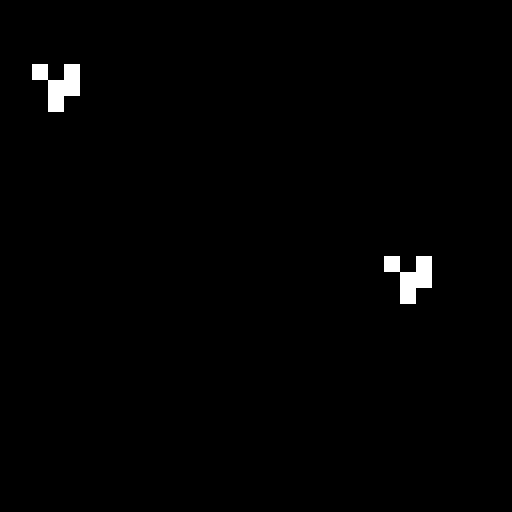
\includegraphics[width=0.15\textwidth]{testout32-1.png}
            
\includegraphics[width=0.15\textwidth]{testout32-2.png}
            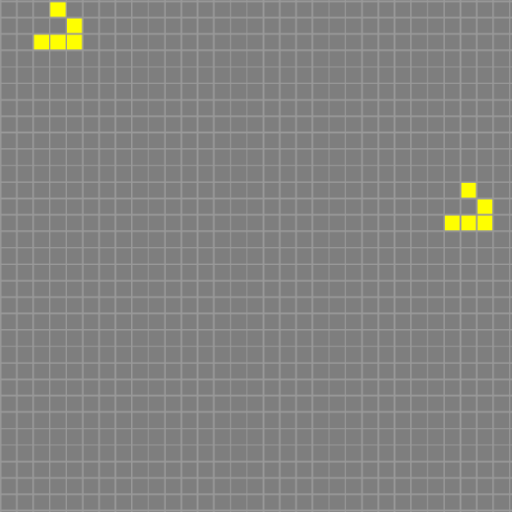
\includegraphics[width=0.15\textwidth]{verify32.png}
            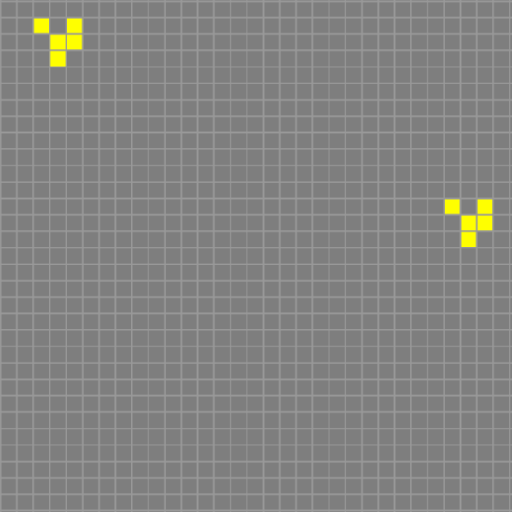
\includegraphics[width=0.15\textwidth]{verify32-1.png}
            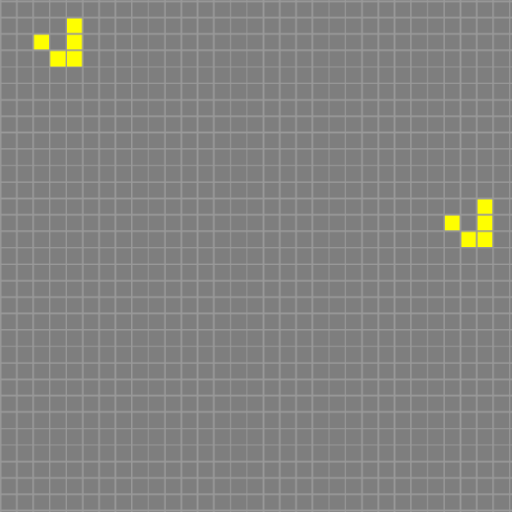
\includegraphics[width=0.15\textwidth]{verify32-2.png}
            \caption{State following 2 iterations of a \texttt{32x32} image. \\ Left: our system; Right: \texttt{https://bitstorm.org/gameoflife/}}
            \label{fig:test32}
        \end{center}
    \end{figure}

    \begin{figure}[h]
        \begin{center}
            
\includegraphics[width=0.2\textwidth]{test1024.png}
            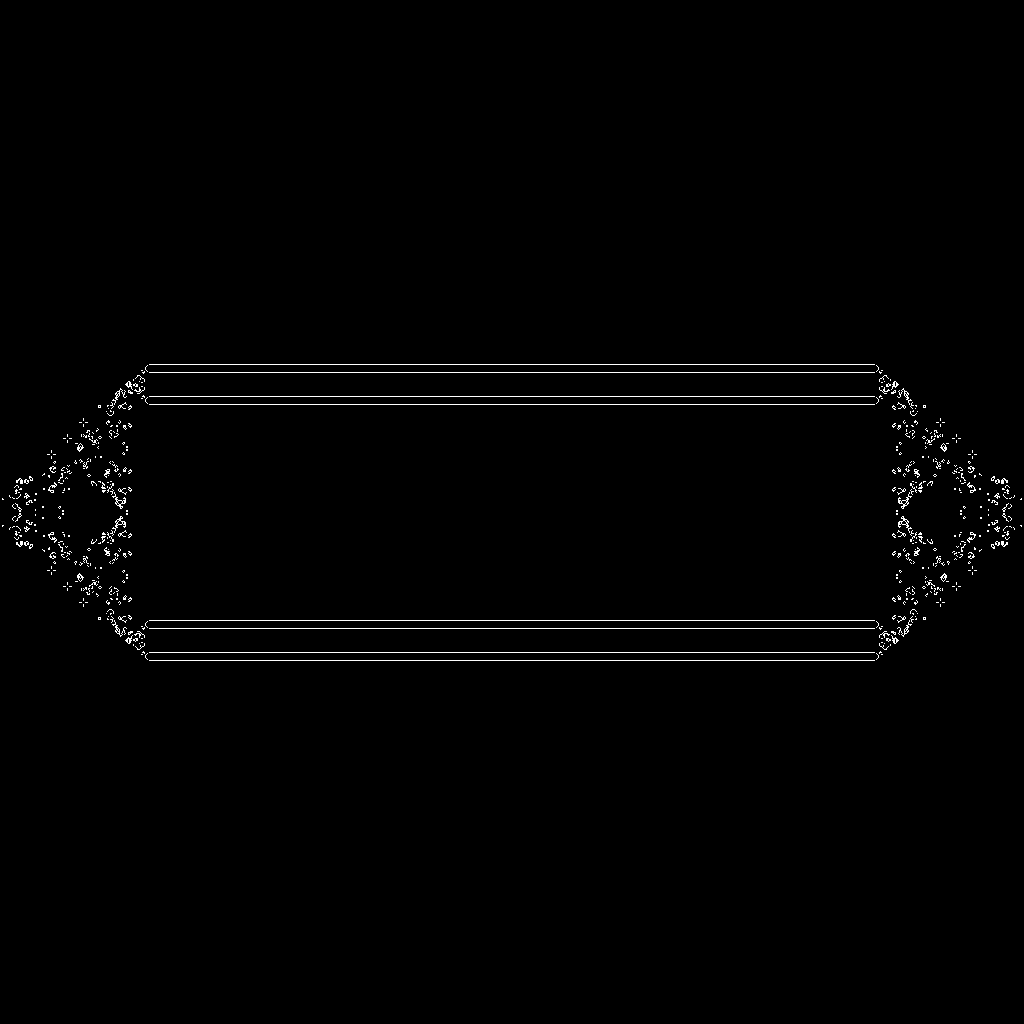
\includegraphics[width=0.2\textwidth]{testout1024-1.png}
            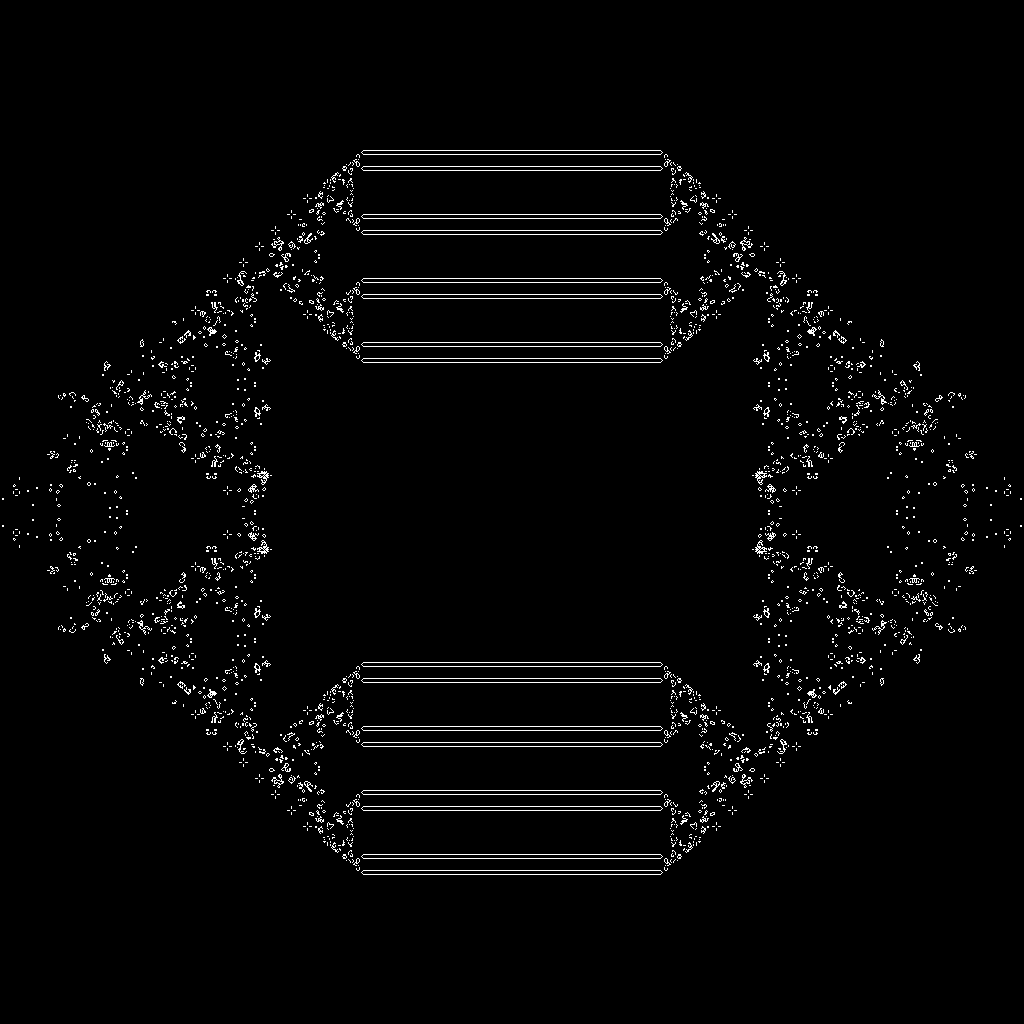
\includegraphics[width=0.2\textwidth]{testout1024-2.png}
            
\includegraphics[width=0.2\textwidth]{testout1024-3.png}
            \caption{Example generations of a \texttt{1024x1024} image, beginning from a straight line.}
            \label{fig:test1024}
        \end{center}
    \end{figure}
    
    \subsection{Worker Count} \label{workercount}

    \begin{figure}[h]
        \begin{center}
            {\small
\begin{tabular}{|c|c|c|c|c|}
    \hline Size & AGT2 (ms) & AGT4 (ms) & AGT8 (ms) \\
    \hline \verb|64x64| & 11.64 & 11.65 & 11.64 \\
    \verb|128x128| & 39.88 & 20.12 & 11.64 \\
    \verb|256x256| & 161.89 & 80.77 & 40.31 \\
    \verb|512x512| & 621.29 & 313.71 & 157.88 \\
    \verb|1024x1024| & 2472.33 & 1250.44 & 622.59 \\
    \hline
\end{tabular}}
            \caption{The effect of increasing worker count and size of image on Average Generation Time.}
            \label{fig:agt}
        \end{center}
    \end{figure}

    \begin{figure}[h]
        \begin{center}
            % This file was created by matplotlib2tikz v0.6.18.
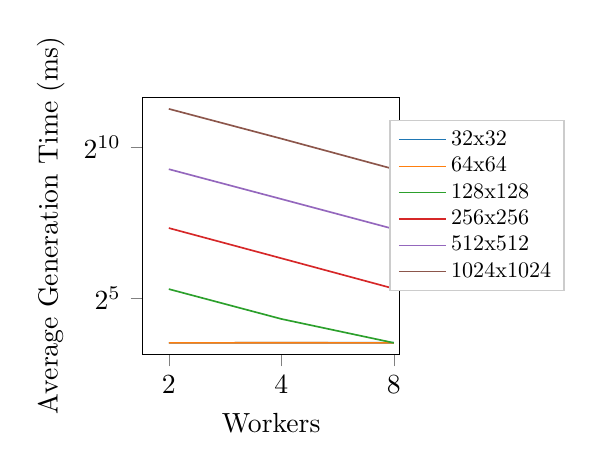
\begin{tikzpicture}

\definecolor{color0}{rgb}{0.12156862745098,0.466666666666667,0.705882352941177}
\definecolor{color1}{rgb}{1,0.498039215686275,0.0549019607843137}
\definecolor{color2}{rgb}{0.172549019607843,0.627450980392157,0.172549019607843}
\definecolor{color3}{rgb}{0.83921568627451,0.152941176470588,0.156862745098039}
\definecolor{color4}{rgb}{0.580392156862745,0.403921568627451,0.741176470588235}
\definecolor{color5}{rgb}{0.549019607843137,0.337254901960784,0.294117647058824}

\begin{axis}[
height=\figureheight,
legend cell align={left},
legend entries={{32x32},{64x64},{128x128},{256x256},{512x512},{1024x1024}},
legend style={nodes={scale=0.8, transform shape}, at={(1.3,0.91)}, anchor=north, draw=white!80.0!black},
tick align=outside,
tick pos=left,
width=\figurewidth,
x grid style={white!69.01960784313725!black},
xlabel={Workers},
xmin=1.7, xmax=8.3,
y grid style={white!69.01960784313725!black},
ylabel={Average Generation Time (ms)},
ymin=8.90420822429587, ymax=3231.94611750847,
ymode=log,
xmode=log,
log basis x={2},
log basis y={2},
xticklabel=\pgfmathparse{2^\tick}\pgfmathprintnumber{\pgfmathresult}
]
\addlegendimage{no markers, color0}
\addlegendimage{no markers, color1}
\addlegendimage{no markers, color2}
\addlegendimage{no markers, color3}
\addlegendimage{no markers, color4}
\addlegendimage{no markers, color5}
\addplot [semithick, color0]
table [row sep=\\]{%
2	11.64 \\
4	11.65 \\
8	11.66 \\
};
\addplot [semithick, color1]
table [row sep=\\]{%
2	11.64 \\
4	11.65 \\
8	11.64 \\
};
\addplot [semithick, color2]
table [row sep=\\]{%
2	39.88 \\
4	20.12 \\
8	11.64 \\
};
\addplot [semithick, color3]
table [row sep=\\]{%
2	161.39 \\
4	80.77 \\
8	40.31 \\
};
\addplot [semithick, color4]
table [row sep=\\]{%
2	621.29 \\
4	313.71 \\
8	157.88 \\
};
\addplot [semithick, color5]
table [row sep=\\]{%
2	2472.33 \\
4	1250.44 \\
8	622.59 \\
};
\end{axis}

\end{tikzpicture}
            \caption{Log plot of Average Generation Time vs. Worker Count.}
            \label{fig:agtplot}
        \end{center}
    \end{figure}

    We can measure the processing speed by the AGT (Average Generation Time). From Figure \ref{fig:agt} it's clear that increasing the number of workers is effective at reducing the AGT, although only up to a point. Regardless of worker count, the AGT for \verb|64x64| and \verb|32x32| remains at 11.64, and the AGT for \verb|128x128| with 8 workers is also 11.64. This implies that there is a bottleneck in our system, either fundamentally by the processor speed or by a design choice of ours.

    However for the larger images, doubling the worker count halves the AGT, which implies that increasing the workers gives a \textit{linear} speed up, and this is reflected by the straight lines in Figure \ref{fig:agtplot}. Furthermore, increasing the image size by a factor of 4 also increases the AGT by a factor of 4; this is expected since an $n$-fold increase in the number of cells is an $n$-fold increase in the amount of work. A nice consequence of this behaviour is that the AGT of an image with $n$ cells and $m$ workers is approximately the same as the AGT of an image with $4n$ cells and $4m$ workers (e.g. the AGT of \verb|128x128| with 2 workers is approximately equal to the AGT of \verb|256x256| with 8 workers).

    \subsection{Worker Distribution} \label{workerdistribution}

    In the \verb|xCore-200| there are \textbf{hard} and \textbf{soft} channels, where hard channels are across physical tiles, and soft channels are between individual threads on a tile. Hard channels will have higher latency since the data must travel a larger distance in comparison to a soft channel. However, using more soft channels means that a single tile is doing more processing, so it may in fact be more efficient to split the work across both tiles to utilise both cores.

    In our experiment we tested \verb|256x256| and \verb|512x512| since they're quick to test while still being large enough to be affected by optimisations.

    \begin{figure}[h]
        \begin{center}
            {\small
\begin{tabular}{|c|c|c|}
    \hline Size & Distribution & AGT (ms) \\
    \hline \verb|256x256| & Distributor and workers on same tile & 80.2 \\
    \verb|256x256| & Distributor and workers on different tiles & 81.37 \\
    \verb|256x256| & Workers split across both tiles & 80.78 \\
    \hline \verb|512x512| & Distributor and workers on same tile & 0 \\
    \verb|512x512| & Distributor and workers on different tiles & 0 \\
    \verb|512x512| & Workers split across both tiles & 0 \\
    \hline
\end{tabular}}
            \caption{The effect of varying the communication between the distributor and workers.}
            \label{fig:hardsoftchannels}
        \end{center}
    \end{figure}

    \subsection{Asynchronous Channels} \label{asyncchannels}

    \pagebreak

    % ?? is a placeholder for a future citation :)
    \section{Critical Analysis} \label{analysis}

    % i've done this wrong :)
\end{document}